\documentclass[12pt, a4paper]{article}

\usepackage[utf8]{inputenc}
\usepackage[russian]{babel}
\parindent 0pt
\parskip 8pt
\usepackage{amsmath}
\usepackage{amssymb}
\usepackage{array}
\usepackage{floatrow}
\usepackage{float}
\usepackage[left=2.3cm, right=2.3cm, top=2.7cm, bottom=2.7cm, bindingoffset=0cm]{geometry}
\usepackage{hyperref}
\usepackage{graphicx}
\usepackage{multicol}
\usepackage{fancyhdr} 
\usepackage{extramarks}
\usepackage[usenames,dvipsnames]{color}
\usepackage{titlesec}
\usepackage{tikz}
\usepackage[T2A]{fontenc} 
\definecolor{grey}{RGB}{128,128,128}

\pagestyle{fancy}
\fancyhf{}
\lhead{Лекция 3}
\chead{Базы данных}
\rhead{\thepage}
\lfoot{by fadyat}
\cfoot{}
\rfoot{22 февраля 2022 г.}
\renewcommand\headrulewidth{0.4pt}
\renewcommand\footrulewidth{0.4pt}


\begin{document}
\section{Иерархическая модель данных}

Задача - хранение деревьев

\subsection{Компоненты иерархической модели}

\begin{itemize}
    \item \emph{Поле данных} -- неделимая, уникально адресуемая единица хранения данных.
    \item \emph{Сегмент данных} -- совокупность полей данных, имеющая уникальную идентификацию.
\end{itemize}

Как правило, поле данных -- атрибут, сегмент данных -- запись, экземпляр данных.

\subsection{Проблемы}

\begin{itemize}
    \item Как оптимально хранить?
    \item Проблема скорости внесения изменений
    \item Дублирование данных
    \item Сложности с контролем целостности данных
    \item Любая реорганизация приводит к трудностям
    \item Невозможность связи - многие ко многим
\end{itemize}

Почему иерархическая модель? Это естественный, нативный способ представления данных.

\newline

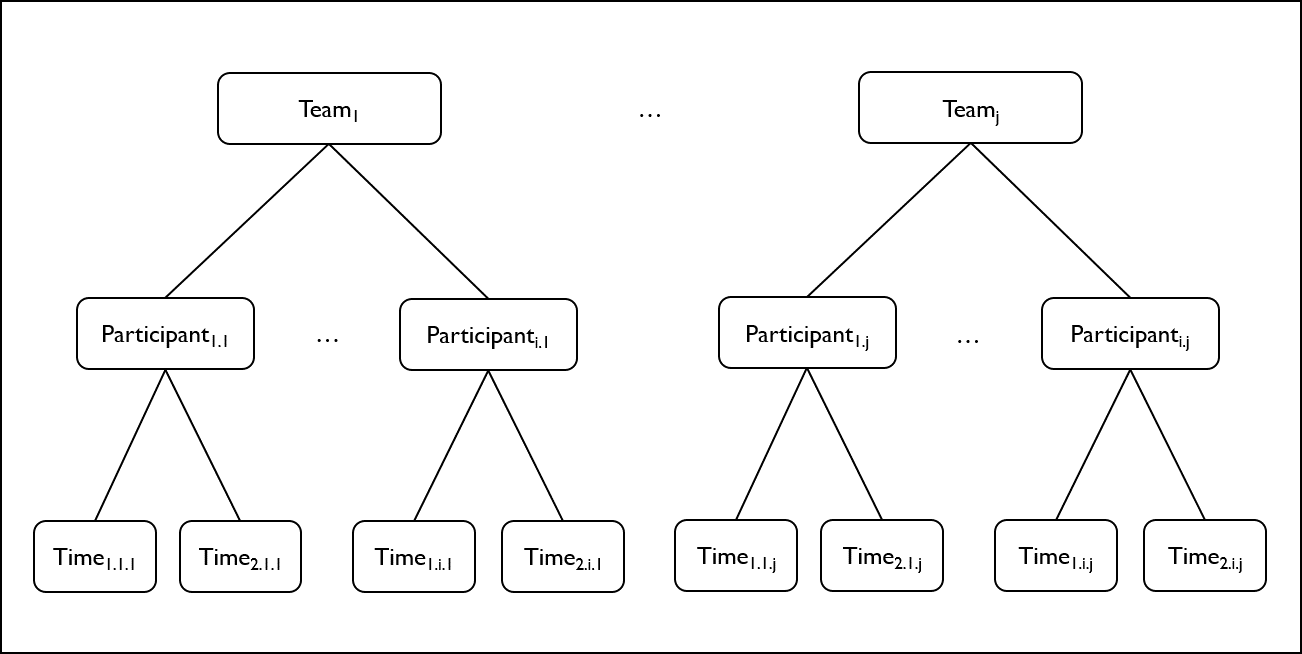
\includegraphics[scale=0.7]{data/hierarchy.jpeg}

\section{Сетевая модель данных}
\subsection{Компоненты сетевой модели}

\begin{itemize}
    \item \emph{Поле данных}
    \item \emph{Агрегат данных} -- совокупность \textbf{множества} полей данных, имеющая уникальную идентификацию
    \item \emph{Связь} -- хранение при помощи ключа, хранение связи = пара ключей + вес
\end{itemize}

\subsection{Новое}

\begin{itemize}
    \item Решает проблемы с дублированием и целостностью данных
    \item Начинаем разделять хранение связей от хранения самих связей
    \item Появление ключей
    \item Возможность связи многие ко многим
\end{itemize}

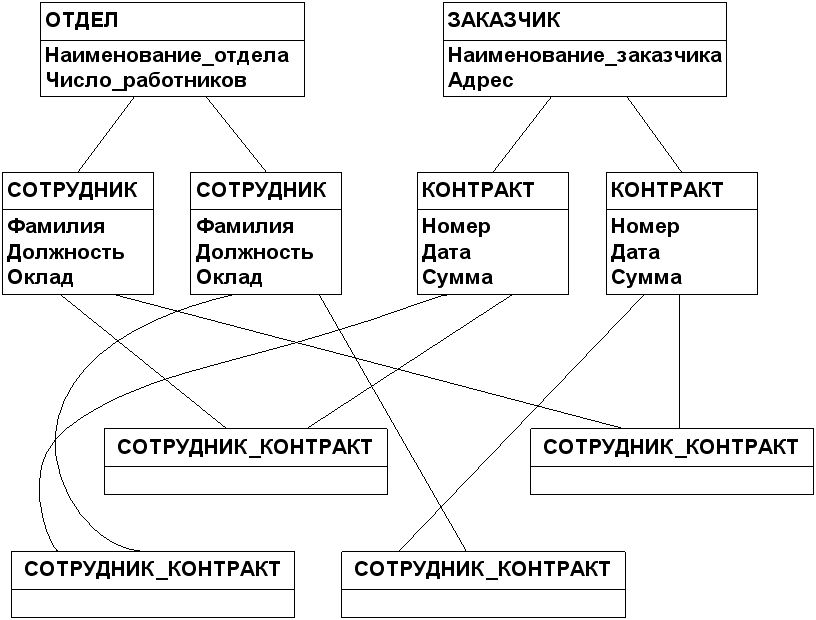
\includegraphics[scale=0.8]{data/network.jpeg}

\subsection{Проблемы}

\begin{itemize}
    \item Дорогое добавление данных, нужно проходить весь граф
    \item Ошибки при хранении пары ключей
\end{itemize}

\section{Реляционная модель данных}

\subsection{Компоненты реляционной модели}

\begin{itemize}
    \item \emph{Поле данных}
    \item \emph{Отношение} -- совокупность множества полей данных (множество кортежей)
    \item \emph{Связь}
\end{itemize}

Реляционная модель -- модель хранения отношений
\begin{itemize}
    \item Один к одному: id
    \item Многие ко многим: новое отношение для хранения связи ключей
\end{itemize}

\subsection{Новое}
Реорганизуем хранение связей - переходим к реляционной модели
\begin{itemize}
    \item Связи хранятся в отдельных отношениях - таблицах
    \item Возникновение предпосылок к избеганию дубликации данных
    \item При грамотной работе гарантируется целостность данных
    \item При грамотной работе гарантирует эффективное время для  выполения записи
    \item При грамотной работе гарантируется отсутствие дубликации данных
\end{itemize}

\subsection{Проблемы}

\begin{itemize}
    \item Поле -- неделимый элемент данных (не имеет внутренней структуры), поэтому возникает проблема с определением типа данных и их хранением
\end{itemize}

\newpage

\section{Постреляционная модель данных}

Снимаем запрет на целостность поля данных - поле данных может само по себе являться агрегатом

\begin{itemize}
    \item При нормализации отношений не гарантируется целостность данных, данные вынесены из понятия отношений
    \item Целостность данных - проблема разработчиков
    \item Проблема больших данных
\end{itemize}

Будем считать, что для нас скорость вычислений важнее памяти.


\section{Многомерная модель}

\begin{itemize}
    \item Многомерное хранение неудобно с точки зрения модификации структуры
    \item OLAP кубы
\end{itemize}

\section{Объектно-ориентированная модель данных}

\subsection{Особенности}
\begin{itemize}
    \item Экземлпяр класса пытаемся сохранить в базе
    \item Улучшается производительность в ООП приложениях
    \item Удобно с точки зрения распределенности систем
\end{itemize}

\subsection{Проблемы}

\begin{itemize}
    \item Замыкаемся на ОО подходе
    \item Целостность данных - обязанность кодовой базы
\end{itemize}

\end{document}
